
\chapter{Medicínska podstata problému} \label{kap:Motivacia}

\pagestyle{fancy}
\fancyhf{}
\fancyfoot[CE,CO]{\thepage}
%\renewcommand{\footrulewidth}{1pt}
\lhead{Medicínska podstata problému}


Spánkové poruchy postihujú približne 30\% svetovej populácie. Podľa súčasnej platnej
medzinárodnej klasifikácie spánkových porúch sú respiračné spánkové poruchy druhým
najčastejšie sa vyskytujúcim ochorením \cite{Sateia_2014}.

Respiračné spánkové apnoické ochorenia delíme na:

\begin{itemize}
	\item \textbf{obštrukčné (OSAS):} dospelí pacienti, pediatrickí pacienti
	\item \textbf{centrálne (CSA):} Cheine-Stokes dýchanie, Primárne, ...
	\item \textbf{zmiešané:} kombinované CSA a OSAS
\end{itemize}

Syndróm obštrukčného spánkového apnoe (OSAS) je respiračná choroba, ktorá spôsobuje
prerušenie oronazálnej ventilácie pri pretrvávajúcom dychovom úsilí na aspoň 10 sekúnd a
opakuje sa viac ako 5 krát za hodinu \cite{Jen_Almeida_Brasher_Doyle-Waters_Salzman_Fleetham_2018}. Na jej vzniku sa vo významnej miere podieľa znížená
priechodnosť horných dýchacích ciest a zmena mechanizmu mäkkých štruktúr horných dýchacích
ciest. Najvýznamnejším rizikovým faktorom vzniku OSAS je anatomické zúženie horných
dýchacích ciest spôsobené predovšetkým: obezitou, kraniofaciálnymi abnormalitami, hypopláziou tváre, zväčšeným objemom mäkkých tkanív, hypertrofiou tonzíl, zväčšením uvuly a dĺžky mäkkého podnebia \cite{Young_Peppard_Gottlieb_2002}.

K presnému stanoveniu OSAS diagnózy sa vykonáva špeciálne komplexné vyšetrenie nazývané
polysomnografia (PSG) \cite{kee2009sleep}. Ide o celonočné monitorovanie pacienta pomocou snímačov a senzorov,
ktoré dávajú lekárovi informáciu o dýchaní, ronchopátii, činnosti srdca, charaktere spánku a jeho jednotlivých cykloch, o polohe tela a o okysličovaní organizmu. PSG sa vykonáva v
akreditovanom spánkovom laboratóriu, ktoré musí byť vybavené potrebnou meracou technikou. Z
výsledkov sa následne určuje konkrétny spôsob liečby \cite{Shrivastava_Jung_Saadat_Sirohi_Crewson_2014}.

PSG je považovaná za štandard pre diagnostiku OSAS, avšak toto vyšetrenie je finančne
nákladné a časovo náročné \cite{hillman2013public}. Navyše na Slovensku ale aj vo svete je problém s nedostatkom spánkových laboratórií, čo spôsobuje dlhé čakacie doby.

Kvôli zníženiu potreby používania PSG adolescentnou skupinou pacientov bol vytvorený
validovaný dotazník nazývaný Klinický záznam o spánku (SCR). Ten pomocou kombinácie
informácií z klinického vyšetrenia, skúmania subjektívnych symptómov pacienta a skúmania
prítomnosti ADHD dokáže s určitou presnosťou identifikovať prítomnosť OSAS. Pozitívni
pacienti sú následne uprednostňovaní na vyšetrenie PSG \cite{Villa}.

Vyšetrenie pomocou kontaktných meracích prístrojov je pre pediatrických pacientov častokrát
stresujúce. Deti sú nepokojné a nedokážu spolupracovať s lekárom, čo predlžuje vyšetrenie a vytvára nepresnosť pri meraní parametrov tváre. Práve z tohto dôvodu vznikla požiadavka na vytvorenie meracieho
systému, ktorý by dokázal zmerať požadované parametre bezkontaktne.

Jedným z možných riešení je vytvorenie skenovacieho zariadenia, ktoré dokáže s určitou
precíznosťou geometricky aj textúrovo zachytiť pacienta. Takto zachytený model môže slúžiť k manuálnej diagnostike bez potreby fyzického kontaktu s pacientom alebo ako vstupné dáta pre algoritmy strojového učenia.

\section{Aktuálny stav výskumu diagnostiky OSAS s použitím 3D dát}

Z dôvodu finančnej a časovej nákladnosti diagnostiky OSAS sa kladie vyšší záujem o vytvorenie skríningového systému, ktorý by vedel identifikovať rizikových pacientov. Aktuálny výskum sa zameriava na predikciu ochorenia z obrazovej informácie. V minulosti a súčastnosti sa diagnostika vykonáva na CT a MRI snímkach, ktorých získanie je komplikované a limitované \cite{Whyte_Gibson_2018}. V posledných rokoch sa pre diagnostiku začalo využívať 3D spracovanie dát. Ich snahou je vytvoriť klasifikačný nástroj, ktorý umožní oddeliť rizikových pacientov od ostatných. 

\newpage
\subsection{Diagnostika pediatrickej OSA prostredníctvom klasifikácie tváre s použitím CNN}

V článku \textit{Diagnosis of Pediatric Obstructive Sleep Apnea via Face Classification with Persistent Homology and Convolutional Neural Networks} \cite{Kiaee2019DiagnosisOP} je opísaná štúdia, v ktorej sa snažia vytvoriť klasifikátor pre rozdelenie vysoko rizikových pacientov od tých menej rizikových. K analýze využívali 3D modely a 2D fotografie obsahujúce snímky týchto 3D objektov. Podľa súčasných štúdií, na ktoré sa v práci odkazujú, využili pre klasifikáciu perzistentnú homológiu (PH) \cite{edelsbrunner2008persistent} a konvolučné neurónové siete (CNN) \cite{szegedy2017inception,szegedy2016rethinking}. Pri prvom prístupe analyzujú trojuholníkové siete cez geometrické príznaky tváre, pri CNN sa pre trénovanie používajú klasifikované 2D obrazy tváre. Použitý dátový set obsahoval 172 detských pacientov. Objekty boli rozdelené lekárom do skupín podľa toho, či patrili do vyššej alebo nižšej rizikovej skupiny OSA. Každý 3D model podstúpil filtráciu (vyplnenie dier v sieti, vyhladenie), pri ktorej sa ale dbalo na to, aby nebola znehodnotená geometrická informácia. 

Z výsledkov PH vyplýva, že súčasné topologické analýzy dát neviedli k presnej klasifikácii. Niektoré rysy tváre síce môžu súvisieť s vysokým rizikom OSA, ale neboli postačujúce pre identifikáciu rizikových pacientov. 


\begin{figure}[h]
	\centering
	\begin{subfigure}[b]{0.32\textwidth}
		\centering
		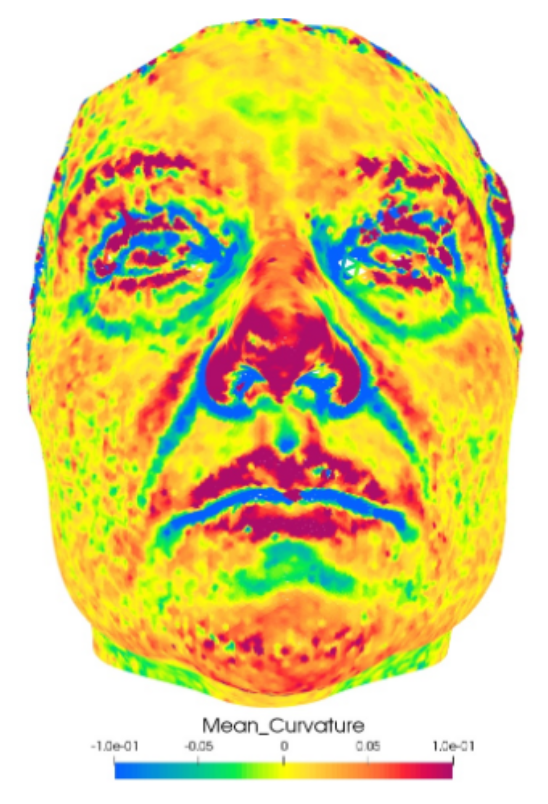
\includegraphics[width=0.95\textwidth]{figures/resers_a.png}
		\caption{}
		\label{fig:resers:a}
	\end{subfigure}
	\hfill
	\begin{subfigure}[b]{0.32\textwidth}
		\centering
		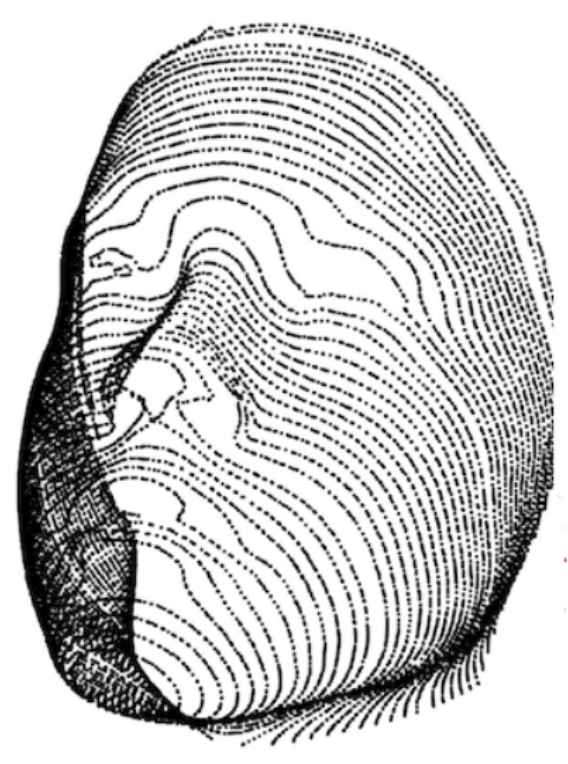
\includegraphics[width=\textwidth]{figures/resers_b.png}
		\caption{}
		\label{fig:resers:b}
	\end{subfigure}
	\hfill
	\begin{subfigure}[b]{0.32\textwidth}
		\centering
		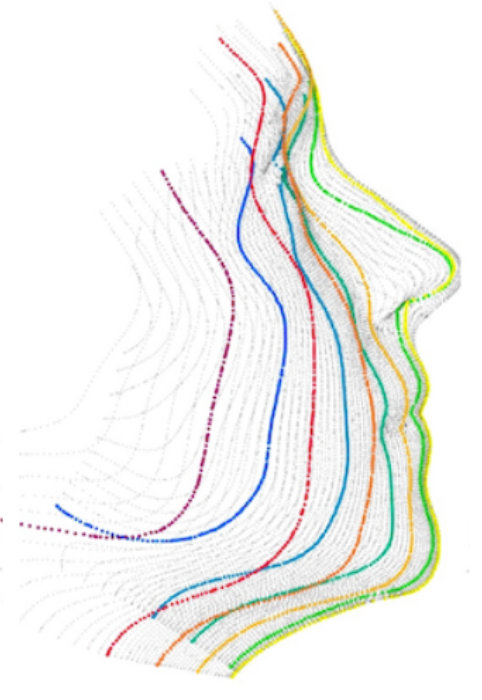
\includegraphics[width=0.95\textwidth]{figures/resers_c.png}
		\caption{}
		\label{fig:resers:c}
	\end{subfigure}
	\caption{Vstupné dáta pre PH klasifikáciu: (\textbf{a}) Priemerné hodnoty zakrivenia pre každý bod v mračne bodov. 
	(\textbf{b}) Krivky tváre
	(\textbf{c}) Geodetika medzi dvoma pacientmi \cite{Kiaee2019DiagnosisOP}. }
	\label{fig:resers:1}
\end{figure}

\newpage


Pre použitie CNN metódy boli z filtrovaných modelov vytvorené série snímok, ktoré zachytávali objekty z rôznych perspektív. Je to kvôli tomu, aby konvolučná neurónová sieť dokázala lepšie pochopiť povrch tváre. Následne boli dáta rozdelené v pomere $80\%$ pre trénovanie a $20\%$ pre testovanie. V článku sa používali CNN architektúry: \textit{InceptionV3}, \textit{InceptionResV2}, \textit{MobileNetV2} a \textit{NASNetLarge}. Tie boli predtrénované na ImageNet datasete. 

Výsledky trénovania pre \textit{MobileNetV2} a \textit{NASNetLarge} sú zobrazené na obr. \ref{fig:resers:d}. Z nich vyplýva, že validácia výstupného modelu nedosahovala očakávané výsledky. 


\begin{figure}[h]
	\centering
	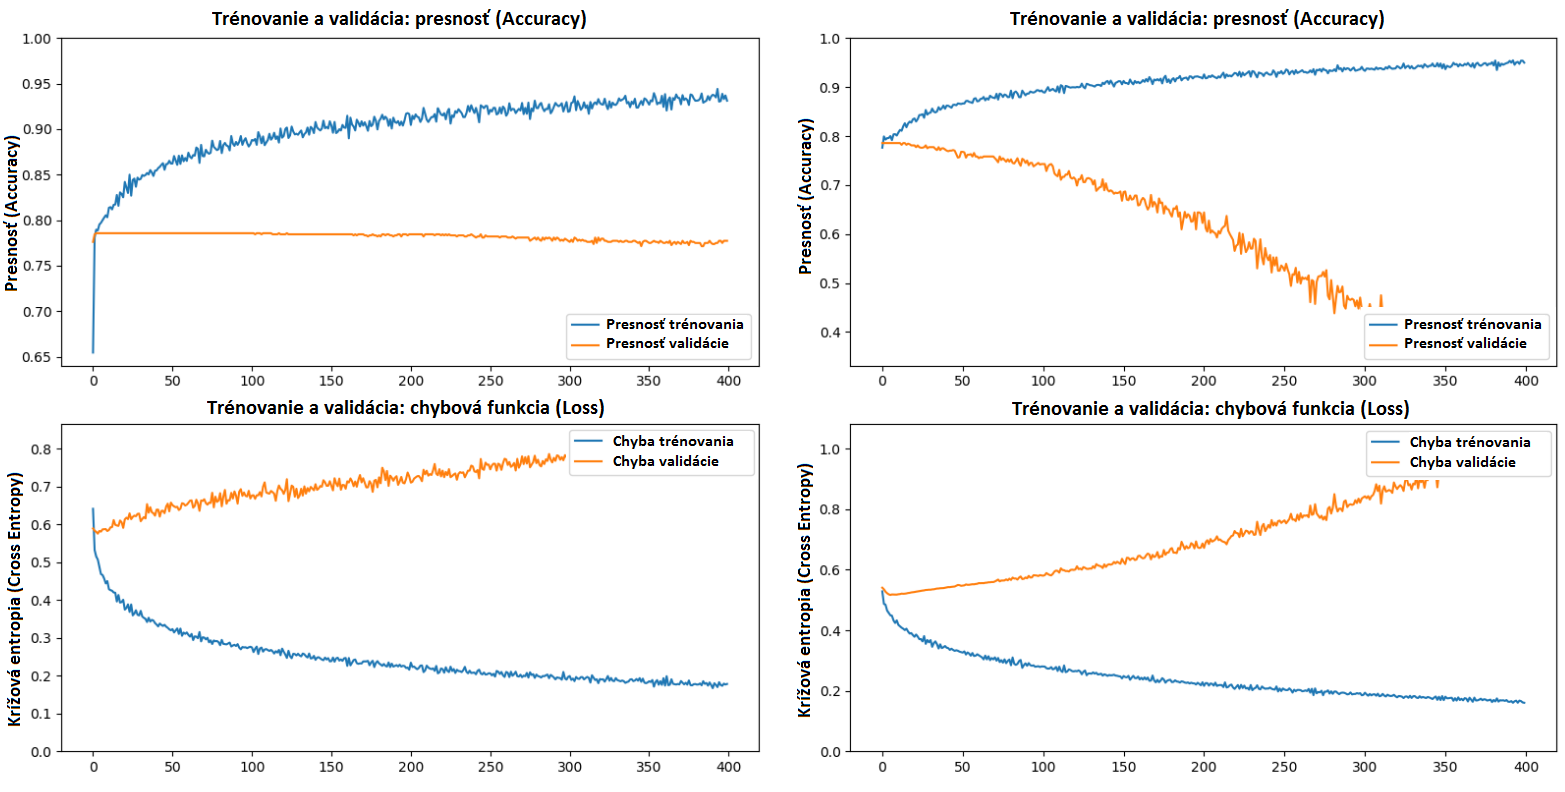
\includegraphics[width=0.9\textwidth]{figures/resers_d.png}
	\caption{Grafy iteračného učenia (školenia a validácie) pre \textit{MobileNetV2} (vľavo) a \textit{NasNetLarge} (vpravo). Spodný riadok ukazuje nákladovosť krížovej entropie a horný presnosť klasifikácie \cite{Kiaee2019DiagnosisOP}.}
	\label{fig:resers:d}
\end{figure}


\begin{table}[H]
	\caption{\label{tab:resers:1} Výsledky validácie predtrénovaných modelov pre použité CNN architektúry \cite{Kiaee2019DiagnosisOP}. }
	\centering
	\begin{tabular}{cccc}
		\toprule
		\textbf{Architektúra} & \textbf{Trénované s} & \textbf{Knižnica} & \textbf{Validácia}     \\ 
		\midrule
		\textbf{InceptionV3}           & ImageNet     	& TensorFlow    & $70 \pm 4$		\\ 
		\textbf{InceptionResV2}        & ImageNet		& TensorFlow  	& $71 \pm 5$		\\ 
		\textbf{MobileNetV2}           & ImageNet     	& TensorFlow    & $64 \pm 5$		\\ 
		\textbf{NASNetLarge}           & ImageNet     	& TensorFlow    & $72 \pm 2$		\\ 
		\bottomrule
	\end{tabular}
\end{table}

Možným dôvodom je, že dátové sety pediatrických OSA pacientov obsahujú malé množstvo klasifikovaných objektov. Ak by sa v budúcnosti vytvorila databáza, ktorá bude zhromažďovať potrebné dáta, je veľký predpoklad na zlepšenie presnosti klasifikovania OSA pacientov pomocou CNN.


\subsection{Predikcia OSA pomocou hlbokého učenia s použitím hĺbkovej mapy tváre}

V článku \textit{Deep Learning of Facial Depth Maps for Obstructive Sleep Apnea Prediction} autori používajú pre detekciu OSA hĺbkové mapy a konvolučné neurónové siete \cite{Islam}. V teoretickom úvode sa odkazujú na súčasné trendy pri diagnostike OSA. Uvádzajú, že nové diagnostické metódy smerujú k využívaniu obrazovej informácii hlavy a krku pacienta \cite{lee2009craniofacial,pae1999shape,lee2009prediction}. V ich práci sa zamerali na využitie hĺbkových máp, ktoré poskytovali informáciu o geometrických parametroch tváre a krku. 

3D dáta boli získané od pacientov, ktorí podstúpili PSG diagnostiku. Databáza bola tvorená z 39 mužských a 30 ženských skenov, ktoré boli vytvorené snímačom Arctec Eva \cite{artec}. Tie boli následne filtrované, čím sa odstránili neželané artefakty (obr. \ref{fig:resers:f}). Z takto upravených modelov boli následne vytvorené 2D hĺbkové mapy (obr. \ref{fig:resers:h}).  

\begin{figure}[h]
	\centering
	\begin{subfigure}[b]{0.62\textwidth}
		\centering
		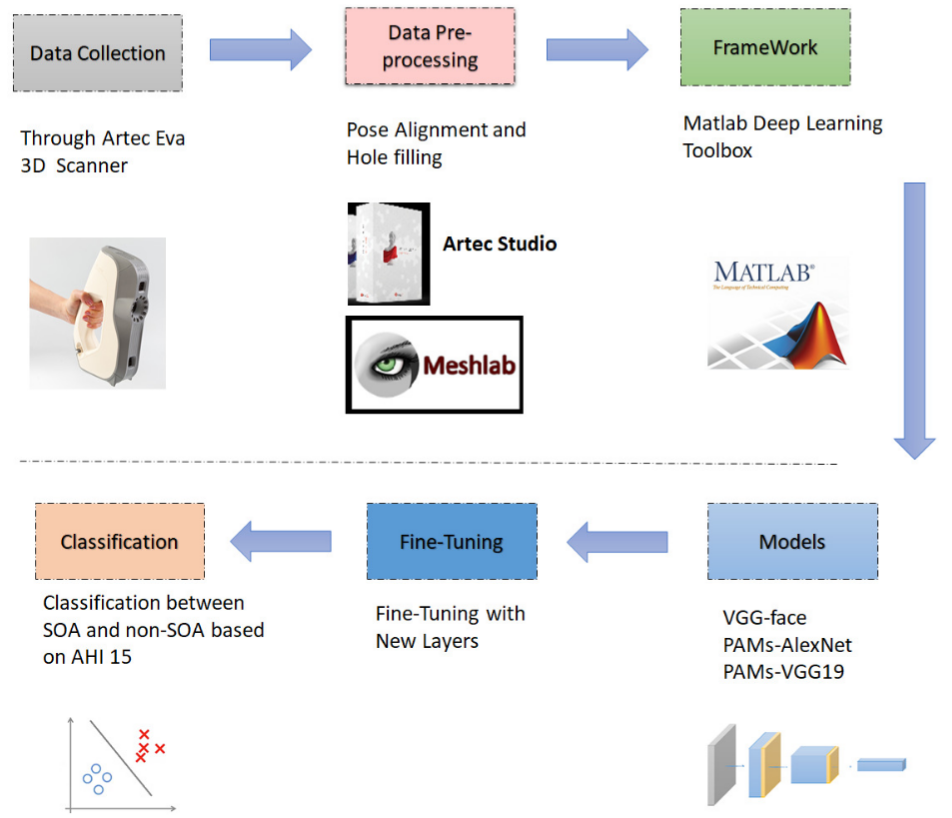
\includegraphics[width=\textwidth]{figures/resers_e.png}
		\caption{}
		\label{fig:resers:e}
	\end{subfigure}
	\hfill
	\begin{subfigure}[b]{0.37\textwidth}
		\centering
		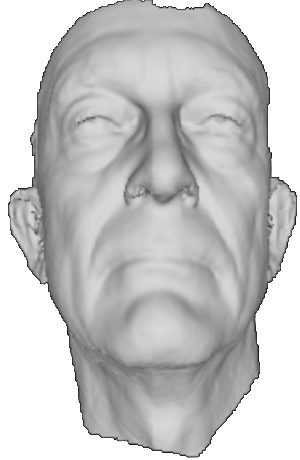
\includegraphics[width=\textwidth]{figures/resers_f.png}
		\caption{}
		\label{fig:resers:f}
	\end{subfigure}
	\caption{(\textbf{a}) Blokový diagram prezentovaného postupu detekcie OSA cez CNN. 
	(\textbf{b}) Ukážka 3D objektu po filtrácii. Tento model bol získaný pomocou laserového skeneru Artec Eva \cite{Islam}.} 
\label{fig:resers:2}
\end{figure}

K trénovaniu si vybrali tri rozdielne neuronové siete, ktoré už boli predtrénované pre detekciu a rozpoznanie tváre. Neboli však trénované na hĺbkových mapách.  \textit{VGG-Face} bol trénovaný na 2.6 miliónovom datasete s presnosťou $ 98.95\% $ \cite{parkhi2015deep}. Taktiež boli vybrané \textit{Pose-Aware CNN} modely \cite{masi2016pose} \textit{AlexNet} \cite{krizhevsky2012imagenet} a \textit{VGG-19} \cite{chatfield2014return}. 
Jemné dolaďovanie modelov sa vykonávalo v \textit{Matlab deep learning toolbox}. Z databázy hĺbkových máp bolo 70\% použitých pre trénovanie (14 modelov na testovanie) a $ 30\% $ pre validáciu. Celý blokový diagram je znázornený na obr. \ref{fig:resers:e}. 

Výsledné modely výstupnej vrstvy po natrénovaní siete s rôznymi vstupnými parametrami sú zobrazené na obr. \ref{fig:resers:g}. Pri PAMs je možné vidieť rôznu aktiváciu očí a nosa na rôznych miestach modelu, pretože model sa musel vysporiadať s rozličnými pózami a natočeniami.  Výstupom \textit{VGG Face} vrstvy je frontálny obraz tváre bez rotácie.

\begin{figure}[h]
	\centering
	\begin{subfigure}[b]{0.195\textwidth}
		\centering
		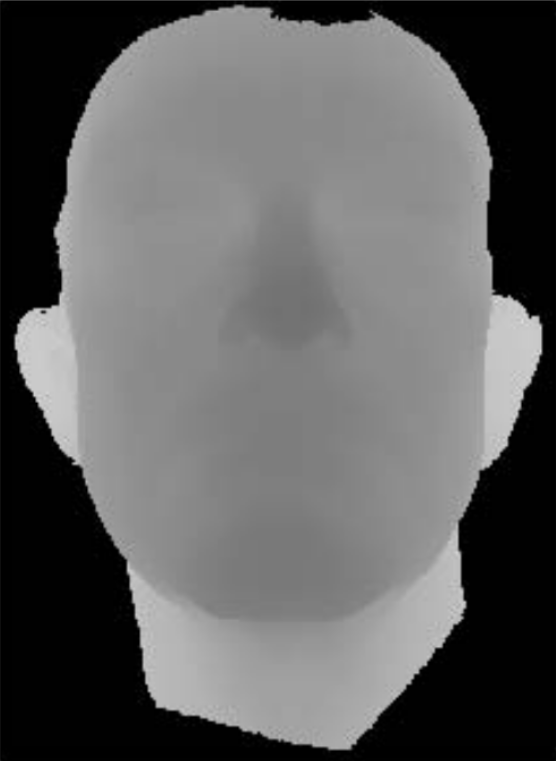
\includegraphics[width=\textwidth]{figures/resers_h.png}
		\caption{}
		\label{fig:resers:h}
	\end{subfigure}
	\hfill
	\begin{subfigure}[b]{0.79\textwidth}
		\centering
		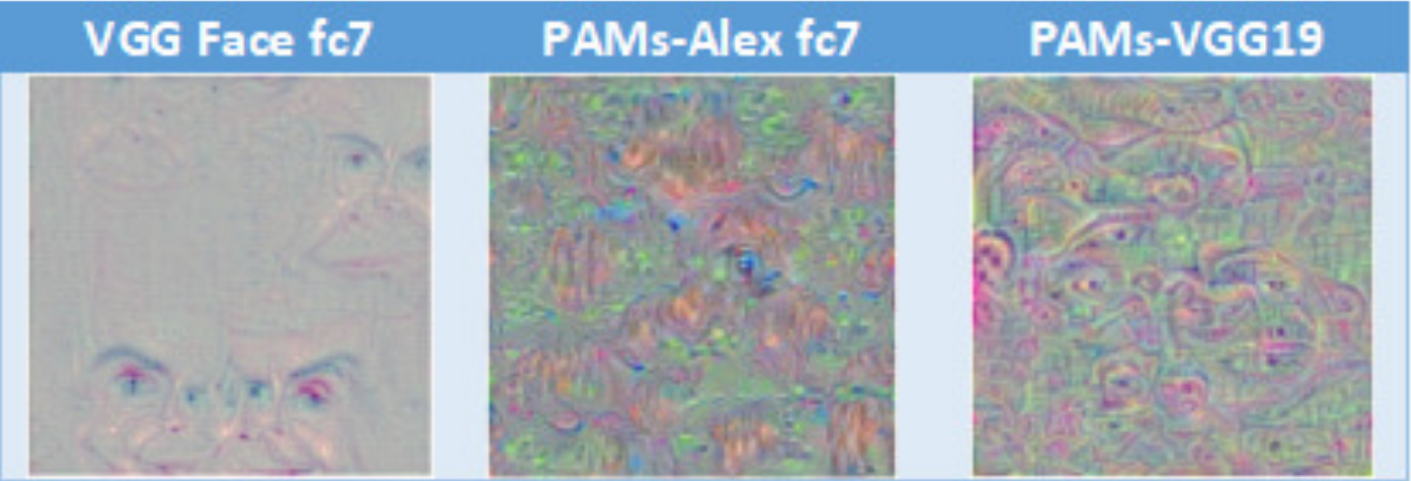
\includegraphics[width=\textwidth]{figures/resers_g.png}
		\caption{}
		\label{fig:resers:g}
	\end{subfigure}
	\caption{(\textbf{a}) Hĺbková mapa získaná z 3D modelu tváre na obr. \ref{fig:resers:f}.
	(\textbf{b}) Vlastnosti vrstvy siete \cite{Islam.}} 
	\label{fig:resers:3}
\end{figure}

Výsledné porovnanie sietí sa nachádza v tabuľke \ref{tab:resers:2}. Z výsledkov vyplýva, že \textit{VGG-Face} dosahovala lepšie výsledky ako \textit{PAMs-VGG19} a \textit{PAMs-Alex}. Jej výhoda je, že bola predtrénovaná na veľkom datasate. 

\begin{table}[H]
	\caption{\label{tab:resers:2} Presnosť klasifikácie použitých modelov. }
	\centering
	\begin{tabular}{cccc}
		\toprule
		\textbf{} & \textbf{VGG Face} & \textbf{PAMs-VGG19} & \textbf{PAMs-Alex}     \\ 
		\midrule
		\textbf{Presnosť validácie}		& 68,75		& 62,5		& 60,15		\\ 
		\textbf{Presnosť testovania}	& 67,42		& 57,14  	& 59,37		\\ 
		\bottomrule
	\end{tabular}
\end{table}

Táto práca predstavuje ako prvá detekciu OSA založenú na hĺbkových mapách. Presnosť klasifikácie, ktorá bola dosiahnutá, je porovnateľná s výsledkami iných prác zaoberajúcich sa detekciou OSA \cite{balaei2017automatic}. Autori článku uvádzajú, že problémom pri trénovaní je malý dátový set hĺbkových máp pacientov. Plánujú jeho rozšírenie a automatizáciu vybraných procesov. 

\subsection{Predikcia OSA pomocou 3D modelu}
\label{sec:med:euclid}
V práci \textit{Predicting Sleep Apnea From Three-Dimensional Face Photography} sa zaoberajú predikciou OSA pomocou lineárnych a geodetických vzdialeností medzi kľúčovými bodmi na tvári \cite{eastwood2020predicting}. Cieľom autorov je nájsť čo najvhodnejšie kombinácie meraní, pre čo najlepšiu predikciu stupňa ochorenia OSA. 
Trojrozmerné snímky prekonávajú limity 2D snímania a pomáhajú určiť štruktúru tkaniva oveľa lepšie ako z 2D fotografie \cite{lin2018three}. Dátový set bol vytvorený zo 400 3D modelov dospelých pacientov, ktorí podstúpili PSG vyšetrenie. Podľa AHI indexu boli pacienti rozdelení do 4 skupín v závislosti od štádia a závažnosti ochorenia. Taktiež bol vypočítaný BMI index a odmeraný obvod krku. 3D modely boli vytvorené kamerou značky 3dMD, ktorá meria vzdialenosť na princípe triangulácie \cite{weinberg2005three,weinberg2006anthropometric}. Pacienti boli pri snímaní naklonený dozadu, aby bola lepšie viditeľná hrdlová časť. Merania lineárnych vzdialeností, uhlov a geodetických vzdialeností boli realizované pomocou anatomických značiek z 3D snímok, z ktorých sa následne určila prítomnosť ochorenia OSA a jeho štádium. Pre detekciu OSA bolo zvolených 24 kľúčových bodov, ktoré boli identifikované v každom 3D modeli (obr. \ref{fig:resers:i}). 


\begin{figure}[h]
	\centering
	\begin{subfigure}[b]{0.44\textwidth}
		\centering
		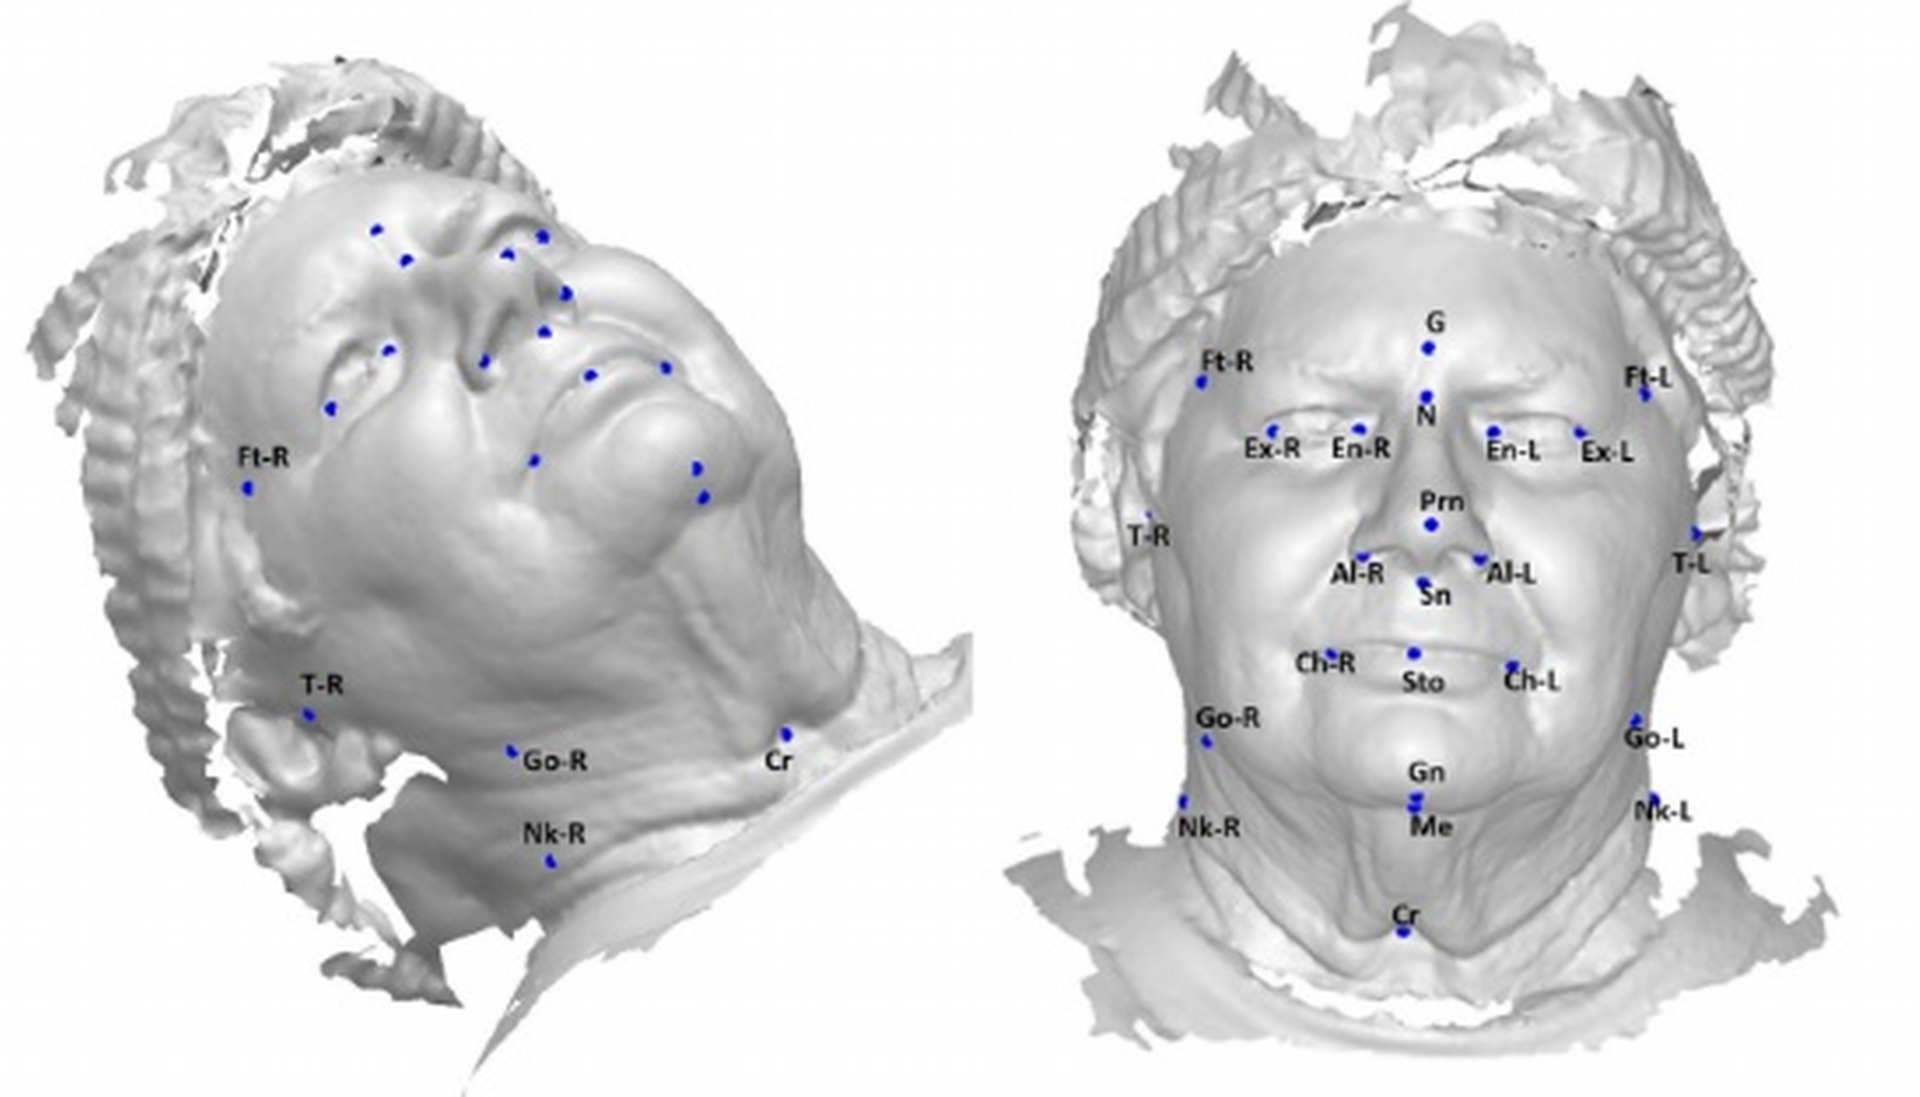
\includegraphics[width=\textwidth]{figures/resers_i.png}
		\caption{}
		\label{fig:resers:i}
	\end{subfigure}
	\hfill
	\begin{subfigure}[b]{0.28\textwidth}
		\centering
		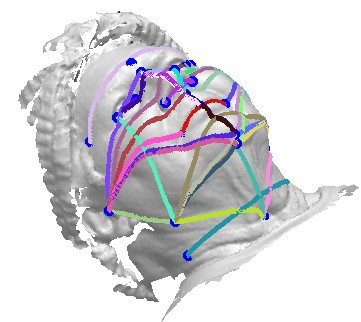
\includegraphics[width=\textwidth]{figures/resers_j.png}
		\caption{}
		\label{fig:resers:j}
	\end{subfigure}
	\hfill
	\begin{subfigure}[b]{0.21\textwidth}
		\centering
		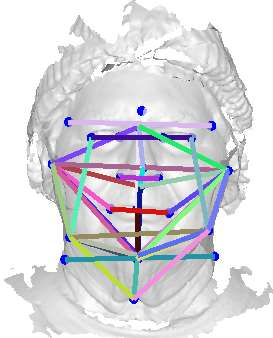
\includegraphics[width=\textwidth]{figures/resers_k.png}
		\caption{}
		\label{fig:resers:k}
	\end{subfigure}
	\caption{(\textbf{a}) Anotované kľúčové body tváre a krku. 
		(\textbf{b}) Geodetické vzdialenosti medzi vybranými pármi bodov.
		(\textbf{c}) Euklidovské vzdialenosti medzi vybranými pármi bodov \cite{eastwood2020predicting}. }
	\label{fig:resers:4}
\end{figure}

Pre detekciu OSA bolo zvolených 24 kľúčových bodov, ktoré boli identifikované v každom 3D modeli \cite{sutherland2016craniofacial,lee2010relationship}. 
Dva z týchto bodov boli vyznačené na tvári pacienta ešte pred skenovaním. Identifikovaním týchto bodov sa získali súradnice $(x,y,z)$, ktoré boli použité pre ďalšiu analýzu. Vďaka týmto súradniciam je možné získať až 276 rôznych vzdialeností medzi dvojicou kľúčových bodov.  Na základe predchádzajúcich štúdií bolo vybraných 25 párov bodov, medzi ktorými boli vypočítané euklidovské a geodetické vzdialenosti. Tieto získané informácie boli použité ako príznaky v ďalšej analýze. 

Na základe prahu $AHI\geq5$ boli vstupné dáta rozdelené na kontrolné (100) a OSA (300). Pomocou tejto hodnoty bol navrhnutý a natrénovaný \textit{Linear Discriminant Analysis} (LDA) algoritmus, ktorý využíval geodetickú vzdialenosť, euklidovskú vzdialenosť a uhol každej snímky. Úlohou algoritmu bolo klasifikovať nové prípady podľa prahu AHI s hodnotami 5, 10, 15, 20, 25, 30, 35, 40, 45 a 50.

Cieľom LDA algoritmu bolo pomocou všetkých popísaných príznakov nájsť 1D priestor, kde vzdialenosť medzi príznakmi v rámci rovnakej triedy bola minimálna a zároveň vzdialenosť medzi príznakmi dvoch odlišných tried maximálna \cite{balakrishnama1998linear}. Dáta boli týmto spôsobom rozdelené do desiatich skupín. Z každej skupiny bolo $ 90\% $ dát použitých na trénovanie a zvyšných 10\% pre testovanie. 

\begin{figure}[h]
	\centering
	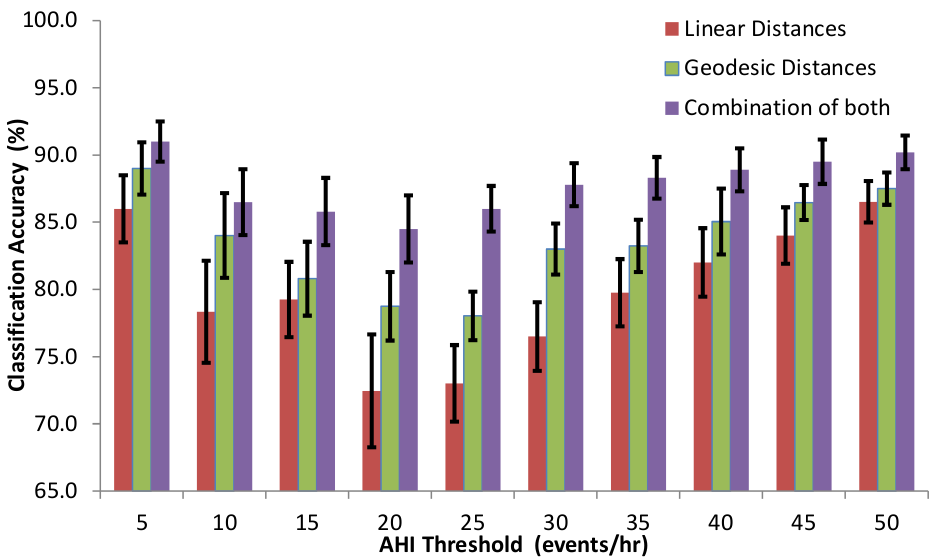
\includegraphics[width=0.7\textwidth]{figures/resers_l.png}
	\caption{Presnosť klasifikácie pre predpovedanie OSA, keď bol algoritmus trénovaný a testovaný pre rozdielne prahové hodnoty AHI (5 až 50) s použitím euklidovskej vzdialenosti (červený stĺpec), geodetickej vzdialenosti (zelený stĺpec) a kombináciu (fialový stĺpec). }
	\label{fig:resers:l}
\end{figure}

Štúdia ukazuje, že geodetická informácia výrazne zlepšuje schopnosť identifikovať rizikových pacientov. Najväčšia presnosť ($ 91\% $) klasifikácie bola získaná pri kombinácií geodetickej a euklidovskej vzdialenosti. Výsledné dáta tejto štúdie nasvedčujú tomu, že 3D skenovanie má potenciálnu úlohu pri skríningu OSA, avšak nedokáže nahradiť PSG vyšetrenie. Z výsledkov taktiež vyplýva, že pomocou geodetickej vzdialenosti je možné určiť aj stupeň závažnosti OSA.

\section{Požiadavky na systém}

Z predchádzajúcej časti vyplýva, že hĺbková informácia môže byť užitočná pri predikcii syndrómu obštrukčného spánkového apnoe (OSAS). Aktuálny výskum sa uberá spracovaním priestorovej informácie, pričom sa využívajú technológie spracovania obrazu a signálov. Z aktuálnych poznatkov nie je úplne zrejme, ktorá metodika je najvhodnejšia pre diagnostiku. 
Aktuálny problém je aj s nedostatkom datasetu OSA pacientov, ktorý by obsahoval 3D informácie. Dôvodom je, že skenovacie zariadenia sú pomerne drahé a doposiaľ neexistuje  plne automatizovaný systém zberu dát. Spánkové laboratóriá sa z týchto dôvodov nezapájajú do spoločného výskumu, ktorý by pomohol k riešeniu celosvetového problému. \newline

Z tohto dôvodu vznikla požiadavka vytvoriť cenovo dostupné zariadenie, ktoré by umožňovalo zachytiť priestorové informácie pacientov. Dôležitým je zosnímanie tváre a krku, pričom sa kladie požiadavka na presnosť. Tá zatiaľ nie je presne špecifikovaná, taktiež nie su pevne špecifikované príznaky. Dôležité je ale minimalizovanie chyby vzniknutej pohybom pri skenovaní. V budúcnosti môže byť špecifikované skenovať tvár pacienta v rôznych polohách a mimikách. \newline

Pri príprave dát sa vykonávalo veľa manuálnych úkonov. Väčšinou išlo o zlepšenie kvality modelov odstraňovaním artefaktov v 3D modeloch. Taktiež sa v niektorých prácach vykonávala manuálna identifikácia kľúčových bodov tváre. Skenovací systém by mal do určitej miery umožňovať automatizáciu procesov. 
